\section{Data}
The data used to train the classifiers was provided by \citeauthor{RN127} \cite{RN127}. 
It was collected between the end of February 2020 and mid of March 2020 from patients admitted to the \textit{IRCSS Ospedale San Raffaele} and consists of 279 individuals who were selected randomly.
For each individual, the data set provides their age, gender, results of a 
routine blood screening, and the result of a PCR test for Sars-CoV-2.
% keep in?
Any other datapoint that could possibly identify the patient, i.e., date of 
admittance or date of PCR test were not recorded.
Table \ref{tab:overview-features} gives an overview over the recorded variables 
in the data set and their variable types. Since the variable \textit{Gender} 
was provided as a string, it was transformed into two binary numerical 
varibales called \textit{female} and \textit{male} by one-hot encoding.
\\
Table \ref{tab:feature-dist} provides common satistics for the numerical 
features of the data set.
\begin{table}[ht]
\centering
\begin{tabular}{lllll}
Feature                          & Unit                    & Mean   & Std    & 
Median \\ \hline
Age                              & Years                   & 61.78  & 17.81  & 
64     \\
White Blood Cell Count (WBC)     & $10^9$/L & 8.55   & 4.86   & 
7.10   \\
Platelets                        & $10^9$/L & 226.5  & 101.2  & 
205.00 \\
Neutrophils                      & $10^9$/L & 6.20   & 4.17   & 
5.10   \\
Lymphocytes                      & $10^9$/L & 1.19   & 0.80   & 
1.00   \\
Monocytes                        & $10^9$/L & 0.61   & 0.41   & 
0.50   \\
Eosinophils                      & $10^9$/L & 0.06   & 0.13   & 
0.00   \\
Basophils                        & $10^9$/L & 0.01   & 0.04   & 
0.00   \\
C-reactive protein (CRP)         & mg/L                    & 90.89  & 94.42  & 
54.20  \\
Aspartate Aminotransferase (AST) & U/L                     & 54.20  & 57.61  & 
36.00  \\
Alanine Aminotransferase (ALT)   & U/L                     & 44.92  & 45.50  & 
31.00  \\
Alkaline Phosphatase (ALP)       & U/L                     & 89.89  & 89.09  & 
71.00  \\
Gamma Glutamyl Transferase (GGT) & U/L                     & 82.48  & 132.70 & 
41.00  \\
Lactate dehydrogenase (LDH)      & U/L                     & 380.45 & 193.98 & 
328.00
\end{tabular}
\caption{Descriptive statistics for numerical features in data set (excluding 
missing values)}
\label{tab:feature-dist}
\end{table}
% non-normality of data with graphs from python as visualization aid
\begin{figure}[ht]
    \centering
    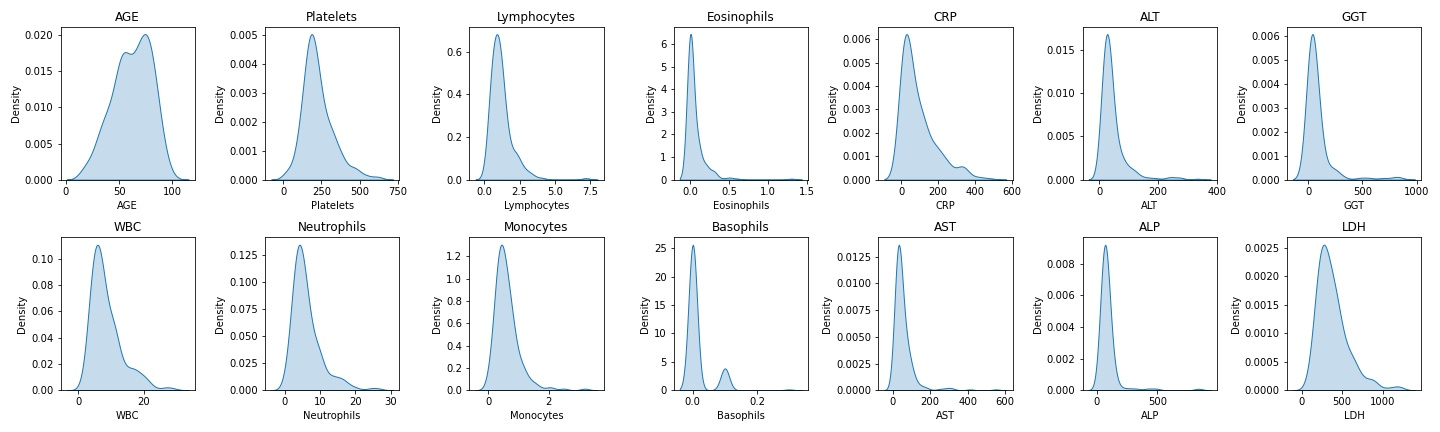
\includegraphics[width=1.1\textwidth]{figures/density_no_split.jpg}
    \caption{Kernel density plots of the numerical features of the data set}
    \label{fig:density}
\end{figure}
\\
As you can see in Figure \ref{fig:density}, most of the data is non-normally 
distributed.
% end with missing values since it's a good transition to MICE

\section{Multivariate Imputation by Chained Equations}
To impute the missing values \citeauthor{RN127} use \textit{Multivariate 
Imputation by Chained Equations} or \textit{MICE} for short. MICE is an 
imputation method proposed by \citeauthor{RN135} \cite{RN135}.
\begin{changemargin}{50pt}{50pt}
Describe MICE algorithm (keine Bewertung, findet in Discussion statt)
\\
Short description of implementation in Python using rpy2
\\
Shortly mention that R implementation is not able to apply MICE model to other 
data only to data it is ``trained''/ ``fitted'' on (or maybe that's for the 
\ref{discussion} Discussion section)
\\
Maybe include PMM?
\end{changemargin}
\section{K-fold nested cross validation}
\section{Classifiers used}
\subsection{Random Forest}
\subsection{Logistic regression}
